
\documentclass[a4paper,12pt]{article}
%%%%%%%%%%%%%%%%%%%%%%%%%%%%%%%%%%%%%%%%%%%%%%%%%%%%%%%%%%%%%%%%%%%%%%%%%%%%%%%%%%%%%%%%%%%%%%%%%%%%%%%%%%%%%%%%%%%%%%%%%%%%%%%%%%%%%%%%%%%%%%%%%%%%%%%%%%%%%%%%%%%%%%%%%%%%%%%%%%%%%%%%%%%%%%%%%%%%%%%%%%%%%%%%%%%%%%%%%%%%%%%%%%%%%%%%%%%%%%%%%%%%%%%%%%%%
\usepackage{eurosym}
\usepackage{vmargin}
\usepackage{amsmath}
\usepackage{graphics}
\usepackage{epsfig}
\usepackage{subfigure}
\usepackage{fancyhdr}

\setcounter{MaxMatrixCols}{10}
%TCIDATA{OutputFilter=LATEX.DLL}
%TCIDATA{Version=5.00.0.2570}
%TCIDATA{<META NAME="SaveForMode"CONTENT="1">}
%TCIDATA{LastRevised=Wednesday, February 23, 201113:24:34}
%TCIDATA{<META NAME="GraphicsSave" CONTENT="32">}
%TCIDATA{Language=American English}

\pagestyle{fancy}
\setmarginsrb{20mm}{0mm}{20mm}{25mm}{12mm}{11mm}{0mm}{11mm}
\lhead{MA4128} \rhead{Kevin O'Brien} \chead{Cluster Analysis  } %\input{tcilatex}

\begin{document}

\section{Clustering Algorithm - Linkage Example}
To better understand how a clustering algorithm works, let’s manually examine
some of the \textbf{\textit{single linkage}} procedure’s calculation steps. We start off by looking at
the initial (Euclidean) distance matrix displayed previously.

\begin{figure}[h!]
	\begin{center}
		% Requires \usepackage{graphicx}
		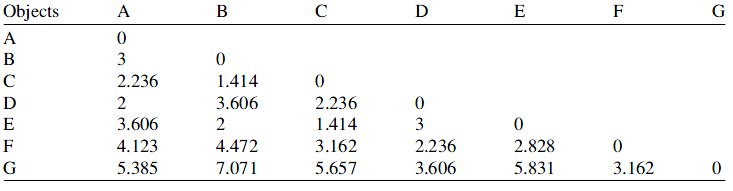
\includegraphics[scale=0.6]{images/DistanceMatrix.jpg}\\
	\end{center}
\end{figure}



\begin{itemize}
	\item In the very first step, the two
	objects exhibiting the smallest distance in the matrix are merged. Note that we
	always merge those objects with the smallest distance, regardless of the clustering
	procedure (e.g., single or complete linkage). (N.B. In the following example, ties will be broken at random.)
	\item As we can see, this happens to two
	pairs of objects, namely B and C ($d(B, C) = 1.414$), as well as C and E ($d(C, E) =
	1.414$). In the next step, we will see that it does not make any difference whether we
	first merge the one or the other, so let’s proceed by forming a new cluster, using
	objects B and C.
	\begin{figure}[h!]
		\begin{center}
			% Requires \usepackage{graphicx}
			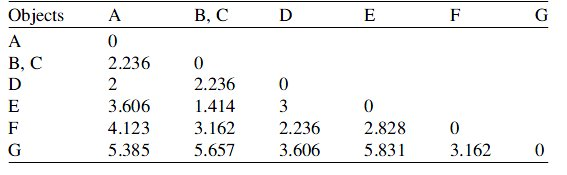
\includegraphics[scale=0.6]{images/DistanceMatrix2.jpg}\\
		\end{center}
	\end{figure}
	\item Having made this decision, we then form a new distance matrix by considering
	the single linkage decision rule as discussed above. According to this rule, the
	distance from, for example, object A to the newly formed cluster is the minimum of
	$d(A, B)$ and $d(A, C)$. As $d(A, C)$ is smaller than $d(A, B)$, the distance from A to the
	newly formed cluster is equal to $d(A, C)$; that is, 2.236.
	\item We also compute the
	distances from cluster [B,C] (clusters are indicated by means of squared brackets)
	to all other objects (i.e. D, E, F, G) and simply copy the remaining distances – such
	as $d(E, F)$ – that the previous clustering has not affected.
	\begin{figure}[h!]
		\begin{center}
			% Requires \usepackage{graphicx}
			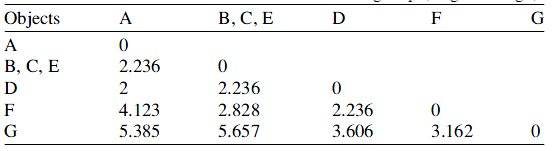
\includegraphics[scale=0.6]{images/DistanceMatrix3.jpg}\\
		\end{center}
	\end{figure}
	\item Continuing the clustering procedure, we simply repeat the last step by merging
	the objects in the new distance matrix that exhibit the smallest distance (in this case,
	the newly formed cluster [B, C] and object E) and calculate the distance from this
	cluster to all other objects.
	\begin{figure}[h!]
		\begin{center}
			% Requires \usepackage{graphicx}
			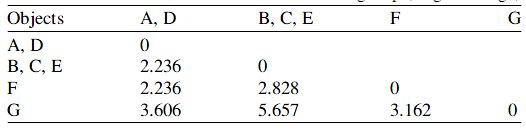
\includegraphics[scale=0.6]{images/DistanceMatrix4.jpg}\\
		\end{center}
	\end{figure}

	\begin{figure}[h!]
		\begin{center}
			% Requires \usepackage{graphicx}
			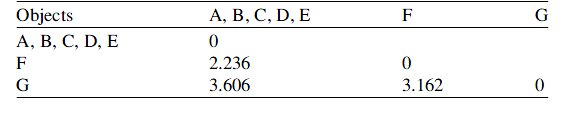
\includegraphics[scale=0.6]{images/DistanceMatrix5.jpg}\\
		\end{center}
	\end{figure}
	\item We continue in the same fashion until one cluster is left. By following the single linkage procedure, the last steps involve the merger
	of cluster [A,B,C,D,E,F] and object G at a distance of 3.162.	\begin{figure}[h!]
		\begin{center}
			% Requires \usepackage{graphicx}
			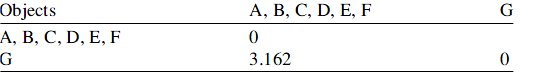
\includegraphics[scale=0.6]{images/DistanceMatrix6.jpg}\\
		\end{center}
	\end{figure}
\end{itemize}
\newpage


\section{Dendrograms}
\begin{itemize}
	
	\item A common way to visualize the cluster analysis’s progress is by drawing a
	dendrogram, which displays the distance level at which there was a combination
	of objects and clusters.
	Here is an example of a dendrogram (which corresponds to the example in the next section of material.
	
	
	\begin{figure}[h!]
		\begin{center}

			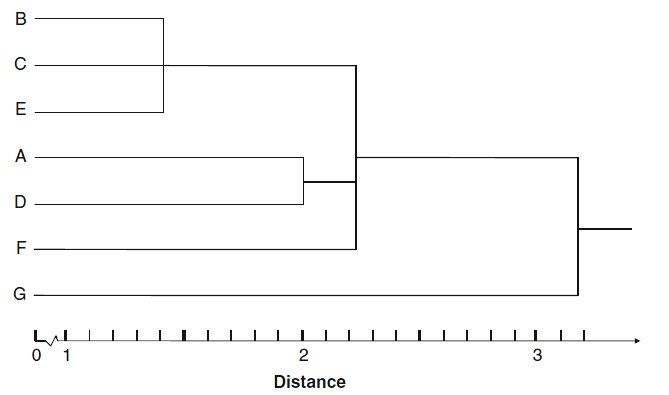
\includegraphics[scale=0.6]{images/Dendrogram.jpg}\\
		\end{center}
	\end{figure}
	
	\item An important question is how to decide on the number of
	clusters to retain from the data. Unfortunately, hierarchical methods provide only
	very limited guidance for making this decision. The only meaningful indicator
	relates to the distances at which the objects are combined. Similar to factor
	analysis’s scree plot, we can seek a solution in which an additional combination
	of clusters or objects would occur at a greatly increased distance. This raises the
	issue of what a great distance is, of course. For this purpose, we can make use of the dendrogram.
	
	\item In constructing the dendrogram, SPSS rescales the distances to a range of 0–25; that is, the last merging step to a one-cluster solution takes place at a
	(rescaled) distance of 25. The rescaling often lengthens the merging steps, thus
	making breaks occurring at a greatly increased distance level more obvious. Despite this, this distance-based decision rule does not work very well in all
	cases.
	
	It is often difficult to identify where the break actually occurs. This is also
	the case in our example above. By looking at the dendrogram, we could justify
	a two-cluster solution ([A,B,C,D,E,F] and [G]), as well as a five-cluster solution
	([B,C,E], [A], [D], [F], [G]).
	
	
	\item 
	The clustering algorithm is based on a distance measure that gives the best results if all variables are independent, continuous variables have a normal distribution (or categorical variables have a multinomial distribution). This is seldom the case in practice, but the algorithm is thought to behave reasonably well when the assumptions are not met.
	
	\item 
	Because cluster analysis does not involve hypothesis testing and calculation of observed significance levels, other than for descriptive follow-up, it's perfectly acceptable to cluster data that may not meet the assumptions for best performance.
	\item 
	The final outcome may depend on the order of the cases in the file. To minimize the effect, arrange the cases in random order. Sort them by the last digit of their ID numbers or something similar.
\end{itemize}



\end{document}

